\documentclass[UTF8,12pt]{article}
\usepackage{ctex}
\usepackage{indentfirst}
\usepackage{color}
\usepackage{hyperref}
\usepackage{graphicx}
\usepackage{subfigure}
\usepackage{pdfpages}
\usepackage{booktabs}
\usepackage{listings}
\hypersetup{
    hidelinks,
	colorlinks=true,
	allcolors=black,
	pdfstartview=Fit,
	breaklinks=true
}

\definecolor{dkgreen}{rgb}{0,0.6,0}
\definecolor{gray}{rgb}{0.5,0.5,0.5}
\definecolor{mauve}{rgb}{0.58,0,0.82}

\lstset{ %
  language=Octave,                % the language of the code
  basicstyle=\footnotesize,           % the size of the fonts that are used for the code
  numbers=left,                   % where to put the line-numbers
  numberstyle=\tiny\color{gray},  % the style that is used for the line-numbers
  stepnumber=2,                   % the step between two line-numbers. If it's 1, each line 
                                  % will be numbered
  numbersep=5pt,                  % how far the line-numbers are from the code
  backgroundcolor=\color{white},      % choose the background color. You must add \usepackage{color}
  showspaces=false,               % show spaces adding particular underscores
  showstringspaces=false,         % underline spaces within strings
  showtabs=false,                 % show tabs within strings adding particular underscores
  frame=single,                   % adds a frame around the code
  rulecolor=\color{black},        % if not set, the frame-color may be changed on line-breaks within not-black text (e.g. commens (green here))
  tabsize=2,                      % sets default tabsize to 2 spaces
  captionpos=b,                   % sets the caption-position to bottom
  breaklines=true,                % sets automatic line breaking
  breakatwhitespace=false,        % sets if automatic breaks should only happen at whitespace
  title=\lstname,                   % show the filename of files included with \lstinputlisting;
                                  % also try caption instead of title
  keywordstyle=\color{blue},          % keyword style
  commentstyle=\color{dkgreen},       % comment style
  stringstyle=\color{mauve},         % string literal style
  escapeinside={\%*}{*)},            % if you want to add LaTeX within your code
  morekeywords={*,...}               % if you want to add more keywords to the set
}


\setlength{\parindent}{2em}

\begin{document}



\begin{center}
    \tableofcontents
\end{center}
\newpage

\section{实验目的}
\begin{enumerate}
    \item 熟悉大型数据库实验环境,以MS SQL SERVER为例
    \item 掌握视图
    \item 掌握存储过程与触发器
    \item 掌握MS SQL SERVER的导入和导出
    \item 掌握MS SQL SERVER的索引
\end{enumerate}

\section{实验内容}
\subsection{创建视图}
使用“实验一”中的数据库“abc”,创建一个视图,生产厂家为“北京”且价格低于北京生产的产品的平均价格,输出产品的名称、价格和生产厂家

\subsection{创建存储过程}
使用“实验一”中的数据库“abc”,创建一个带有输入参数的存储过程proc\_abc,查询指定职工的销售记录,用户输入职工编号,存储过程返回职工名称、产品名称、销售日期、销售数量,假如执行存储过程时所提供的“职工编号”不存在,存储过程应给予一定的提示

\subsection{练习使用游标}
使用“实验一”中的数据库“abc”,练习使用游标, 写出按如下报表形式显示结果的SQL语句,该报表查询每年每种产品总销售金额,(总销售金额=价格\*销量),报表显示格式如下所示:

\begin{tabular}{ccccc}
    \toprule
    年&产品号&产品名&销售总量&总销售金额(万元)\\
    \midrule
    2001年&2&AAA&590&3.2\\
    2002年&5&BBB&644&23.3\\
    2002年&1&CCC&32&0.2\\
    \bottomrule
\end{tabular}

\subsection{创建触发器}
使用“实验一”中的数据库“abc”,练习使用触发器,在销售表上创建触发器tr\_updateprice,每次新增销售记录时,自动更新产品表的单价,更新方法是:每增加一笔销售记录,就将该产品的单价减去1块钱。

\subsection{创建索引}
将100万行网络连接监控数据Netflow导入数据库,创建多个索引,观察创建索引对数据库文件大小的影响;并设计不同的查询语句来观察索引对查询效率的影响;可以尝试将100万行记录扩展为1000万行,然后再做索引和查询的实验?文件见附件。

\section{实验步骤及结果}
\subsection{创建视图}
使用“实验一”中的数据库“abc”,创建一个视图,生产厂家为“北京”且价格低于北京生产的产品的平均价格,输出产品的名称、价格和生产厂家。

使用create view语句创建视图,代码如下:
\begin{lstlisting}[title=create view,frame=shadowbox]
    create view view1
    as
    select CPM as '产品名',JG as '价格',SCCJ as '生产厂家'
    from CPB
    where SCCJ='北京' and JG<(select AVG(JG) from CPB where SCCJ='北京')
    
    select *
    from view1
\end{lstlisting}

使用视图查询的结果如下:
\begin{figure}[htbp]
    \centering
    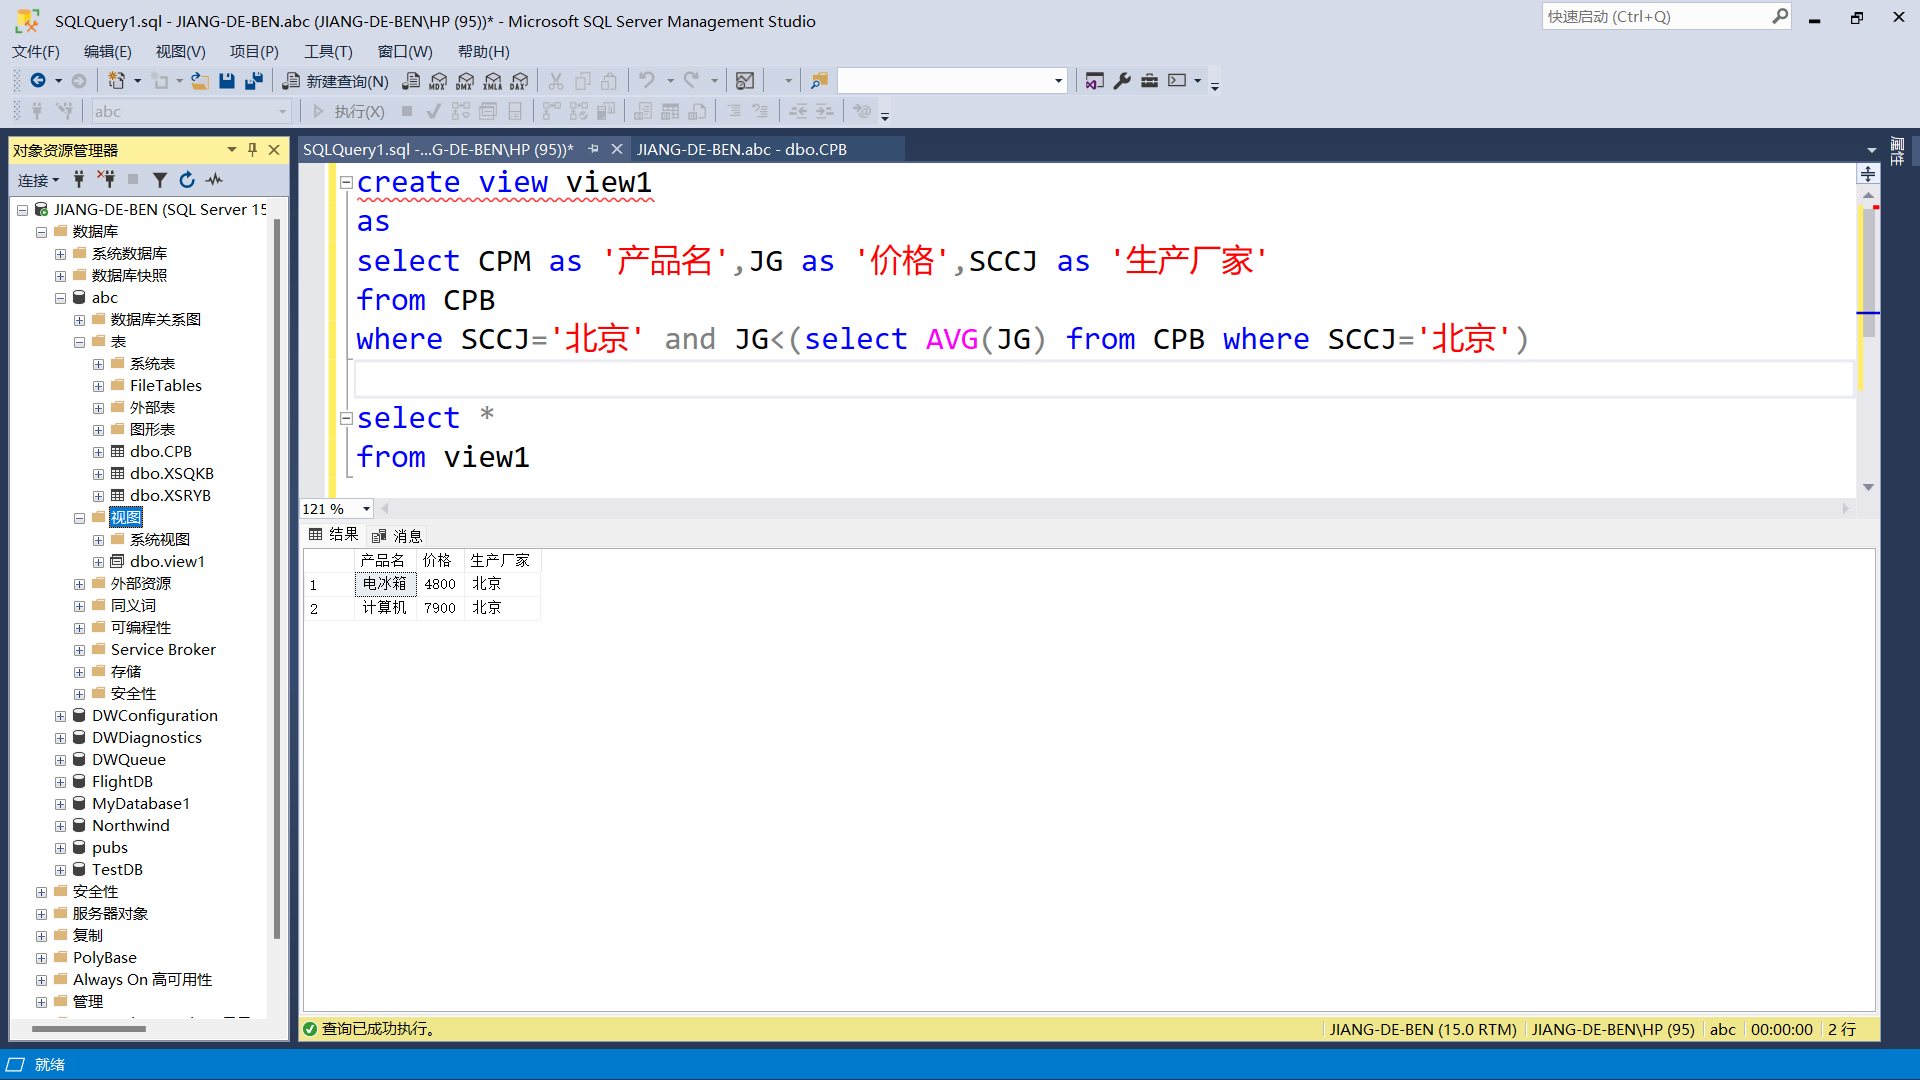
\includegraphics[width=0.8\textwidth]{img/1.png}
    \caption{视图查询结果}
\end{figure}

\subsection{创建存储过程}
使用“实验一”中的数据库“abc”,创建一个带有输入参数的存储过程proc\_abc,查询指定职工的销售记录,用户输入职工编号,存储过程返回职工名称、产品名称、销售日期、销售数量,假如执行存储过程时所提供的“职工编号”不存在,存储过程应给予一定的提示。

使用create procedure语句创建存储过程,代码如下:
\begin{lstlisting}[title=create procedure,frame=shadowbox]
    create procedure proc_abc
    @myzgh char(6)
    as declare @count int
    set @count=
    (
    select count(*)
    from XSRYB
    where ZGH=@myzgh
    )
    if @count>0
    begin
        select XSRYB.XM as '姓名',CPB.CPM as '产品名',XSQKB.XSRQ as '销售日期',XSQKB.XSSL as '销售数量'
        from XSRYB inner join XSQKB on XSRYB.ZGH=XSQKB.ZGH
        inner join CPB on CPB.CPH=XSQKB.CPH
        where XSRYB.ZGH=@myzgh
    end
    else
    begin
        print '查询职工号不存在!'
    end
\end{lstlisting}

使用存储过程查询的结果如下:
\begin{figure}[htbp]
	\centering
	\begin{minipage}{0.4\linewidth}
		\centering
		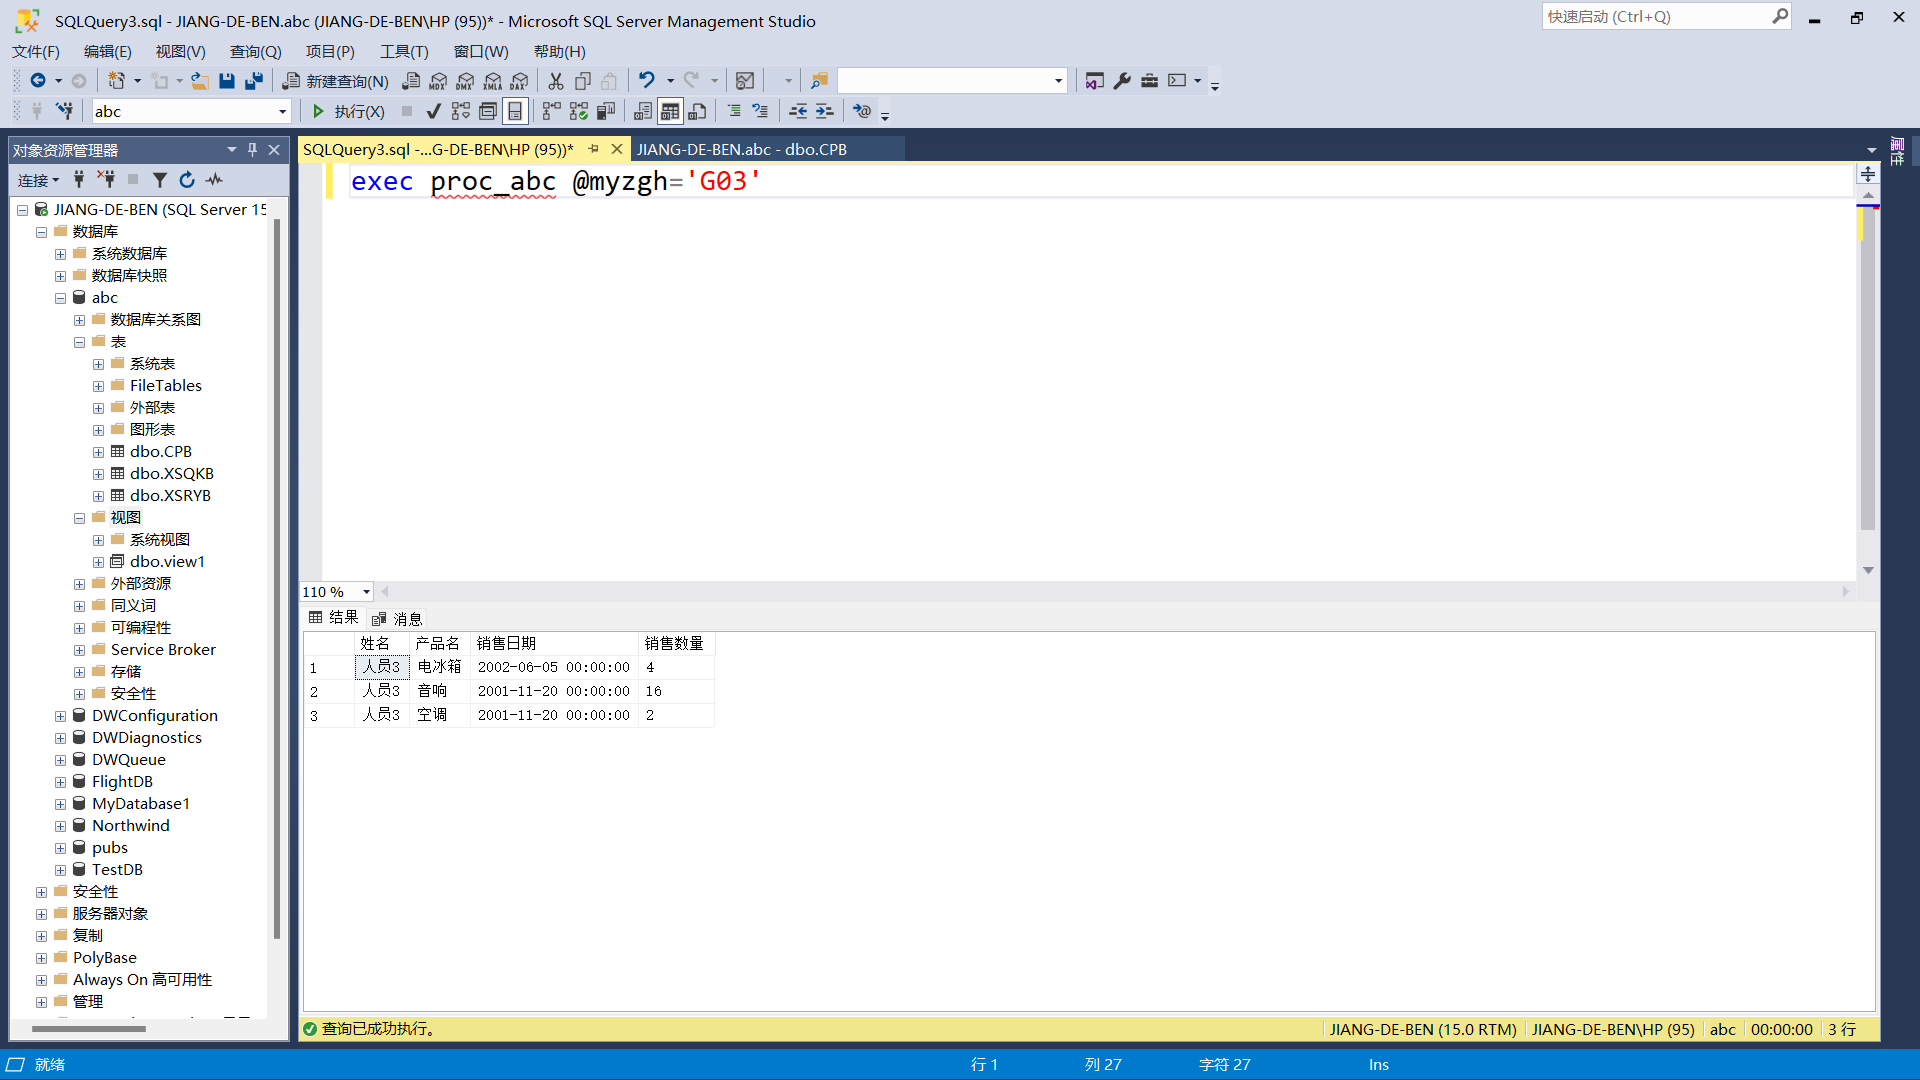
\includegraphics[width=0.9\linewidth]{img/2.png}
	\end{minipage}
	\begin{minipage}{0.4\linewidth}
		\centering
		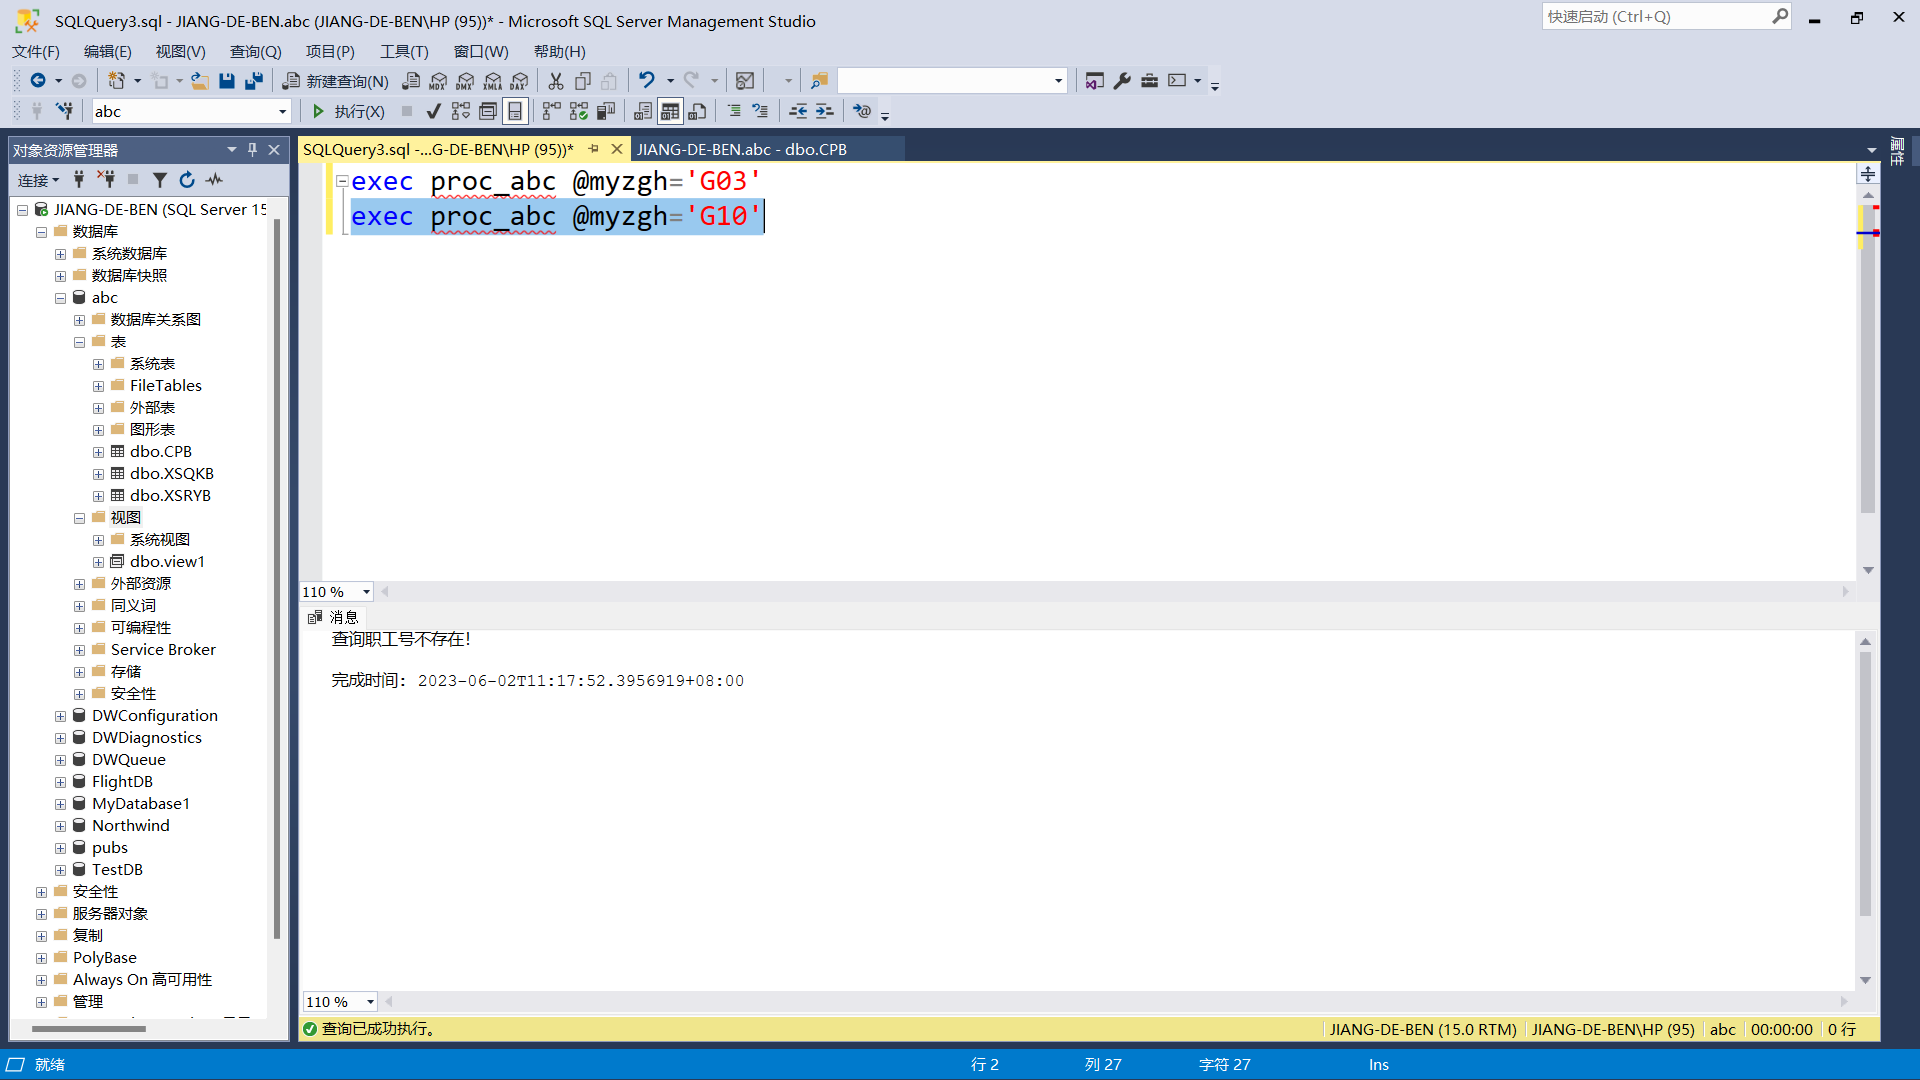
\includegraphics[width=0.9\linewidth]{img/3.png}
	\end{minipage}
    \caption{存储过程查询结果}
\end{figure}

\subsection{练习使用游标}
创建游标的代码如下:
\begin{lstlisting}[title=创建游标,frame=shadowbox]
    declare
	abc_cursor2 cursor for
	select year(XSRQ),CPH
	from XSQKB
	group by year(XSRQ),CPH
\end{lstlisting}

练习使用游标,写出按照上述报表形式显示结果的SQL语句,该报表查询每年每种产品总销售金额,代码如下:
\begin{lstlisting}[title=练习使用游标,frame=shadowbox]
    open abc_cursor2

    declare
        @YEAR int,
        @CPH char(6),
        @CPM varchar(20),
        @XSZL int,
        @ZXSJE float
    
    create table #temp_cursor2
    (
        [year] [int],
        [cph] [char](6),
        [cpm] [varchar](20),
        [xszl] [int],
        [zxsje] [float]
    )on [primary]
    
    fetch next from abc_cursor2
    into @YEAR,@CPH
    
    while @@FETCH_STATUS=0
    begin
        set @XSZL=
        (
            select sum(XSSL)
            from XSQKB
            where CPH=@CPH and year(XSRQ)=@YEAR
        )
    
        set @CPM=
        (
            select CPM
            from CPB
            where CPH=@CPH
        )
    
        set @ZXSJE=
        (
            select JG*@XSZL
            from CPB
            where CPH=@CPH
        )
        insert into #temp_cursor2
        values(@YEAR,@CPH,@CPM,@XSZL,cast((@ZXSJE/10000) as varchar(10)))
        fetch next from abc_cursor2 into @YEAR,@CPH
    end
    
    close abc_cursor2
    deallocate abc_cursor2
    
    select year as '年',cph as '产品号',cpm as '产品名',xszl as '销售总量',zxsje as '总销售金额(万元)'
    from #temp_cursor2
    
    drop table #temp_cursor2
\end{lstlisting}

使用游标查询的结果如下:
\begin{figure}[htbp]
    \centering
    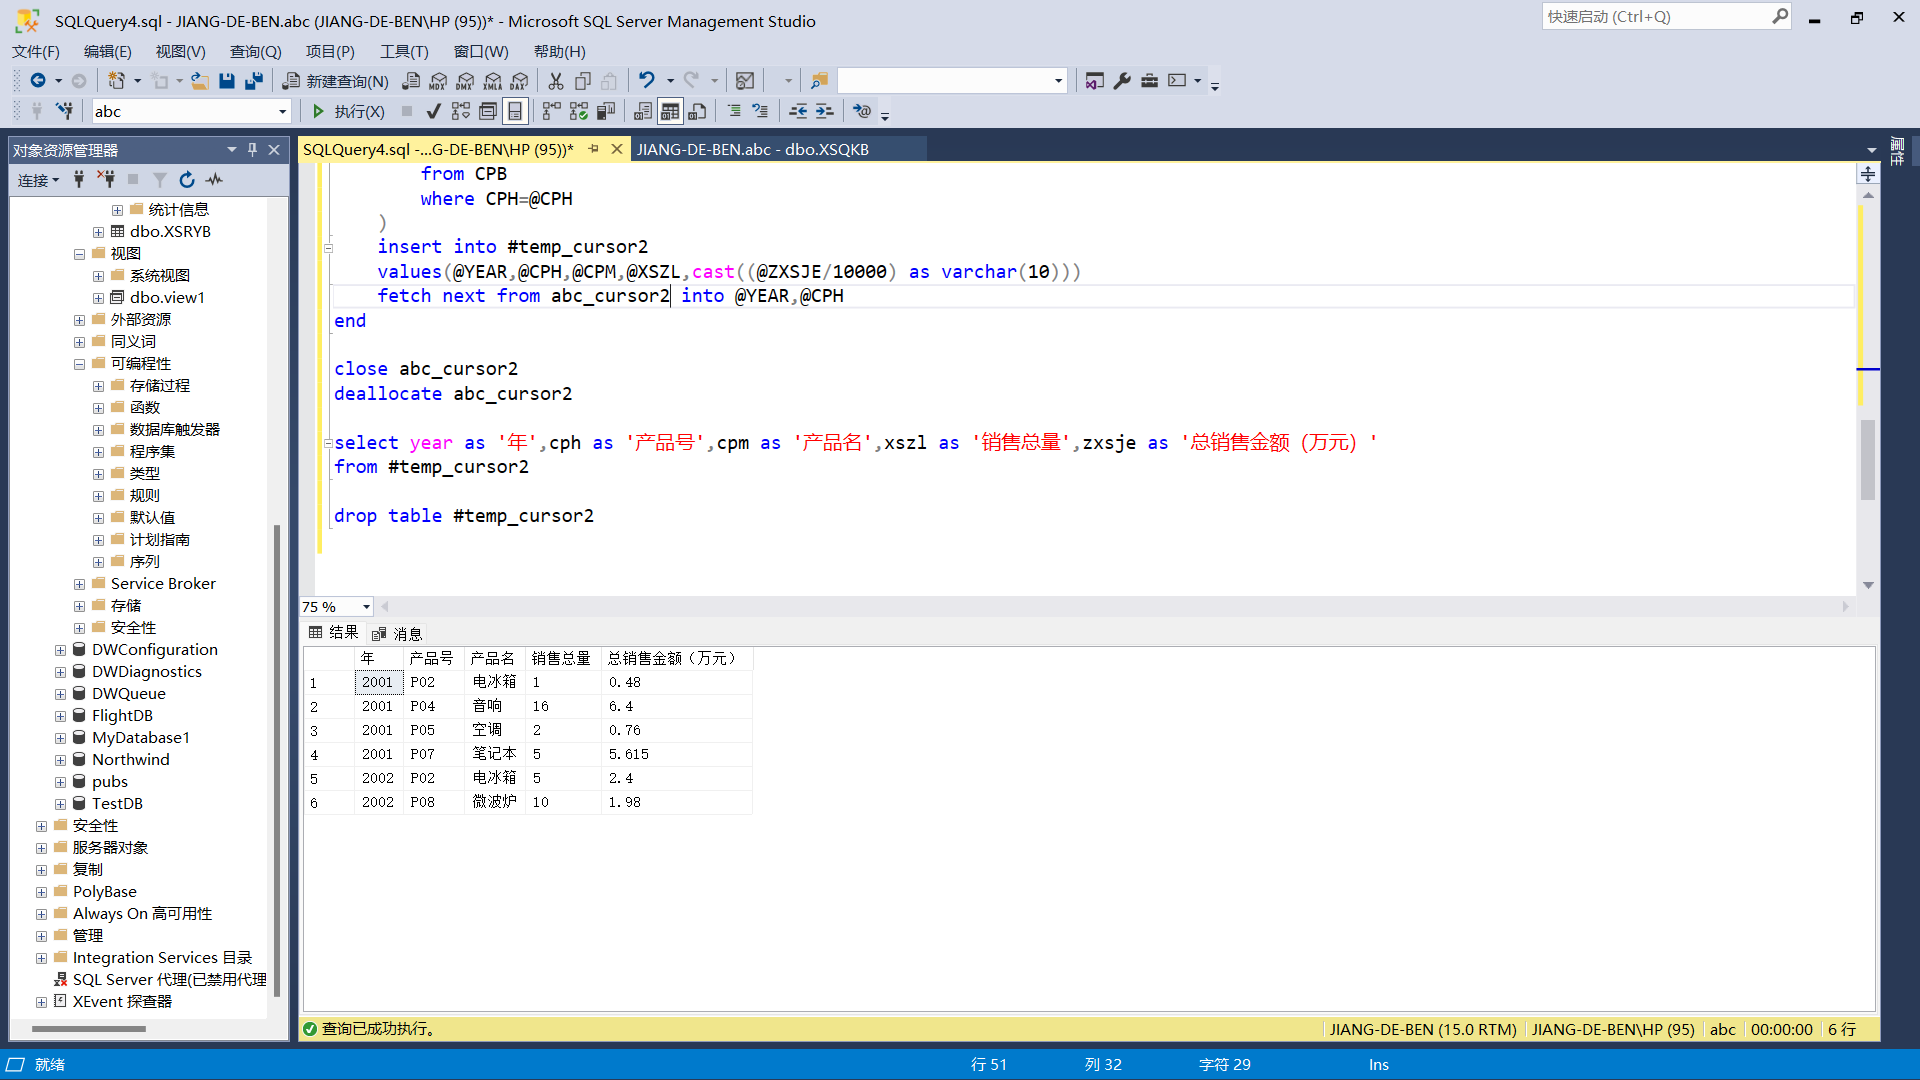
\includegraphics[width=0.8\textwidth]{img/4.png}
    \caption{游标查询结果}
\end{figure}

\subsection{创建触发器}
使用“实验一”中的数据库“abc”,练习使用触发器,在销售表上创建触发器tr\_updateprice,每次新增销售记录时,自动更新产品表的单价,更新方法是:每增加一笔销售记录,就将该产品的单价减去1块钱。

创建触发器的代码如下:
\begin{lstlisting}[title=创建触发器,frame=shadowbox]
    create trigger tr_updateprice
    on XSQKB
    for insert,update
    as
    declare
        @newXSSL int,
        @newJGCPH char(6)
    
    set @newXSSL=(select XSSL from inserted)
    set @newJGCPH=(select CPH from inserted)
    
    update CPB
    set JG=JG-@newXSSL
    where CPH=@newJGCPH
\end{lstlisting}

使用触发器的代码如下:
\begin{lstlisting}[title=使用触发器,frame=shadowbox]
    select * from XSQKB
    select * from CPB
    
    insert into XSQKB
    values
    ('G01','P02','2023-5-30',10)
    
    select * from XSQKB
    select * from CPB
\end{lstlisting}

使用触发器查询的结果如下:
\begin{figure}[htbp]
	\centering
	\begin{minipage}{0.49\linewidth}
		\centering
		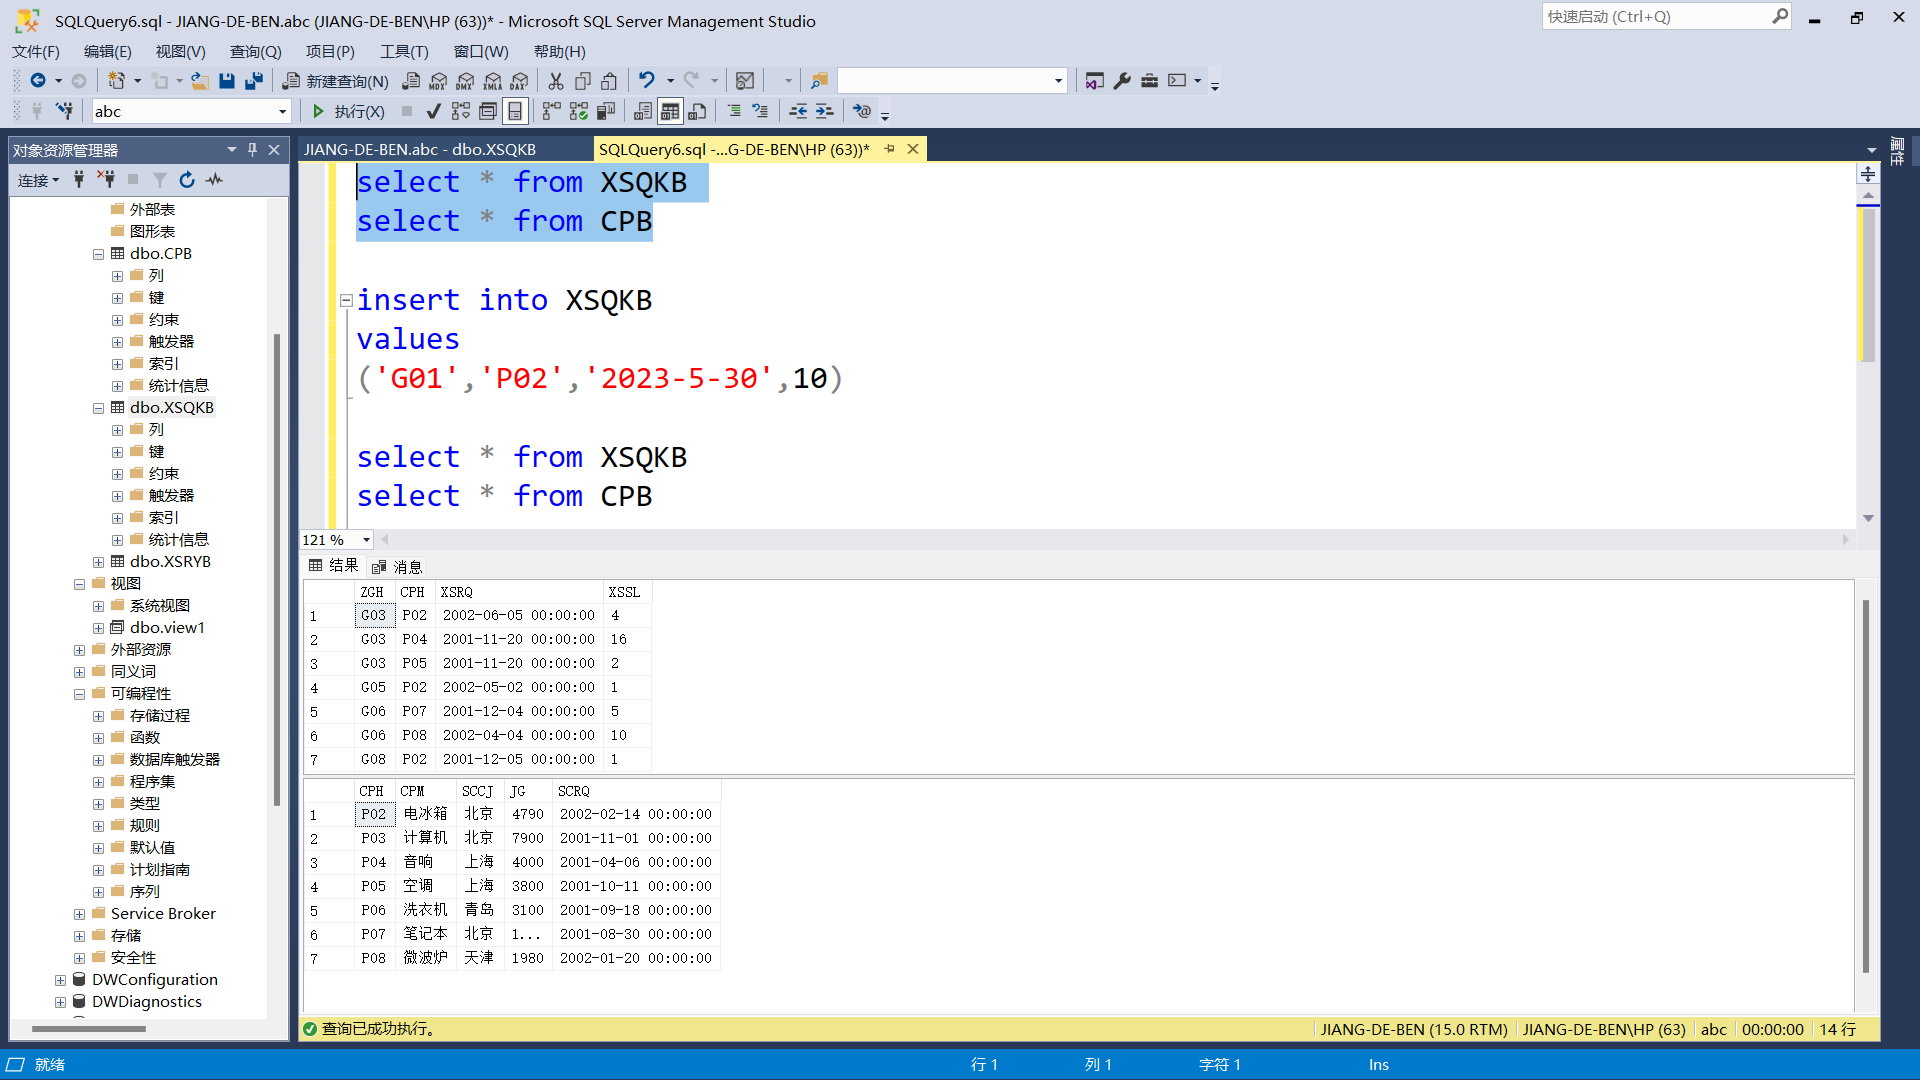
\includegraphics[width=0.9\linewidth]{img/5.png}
	\end{minipage}
	\begin{minipage}{0.49\linewidth}
		\centering
		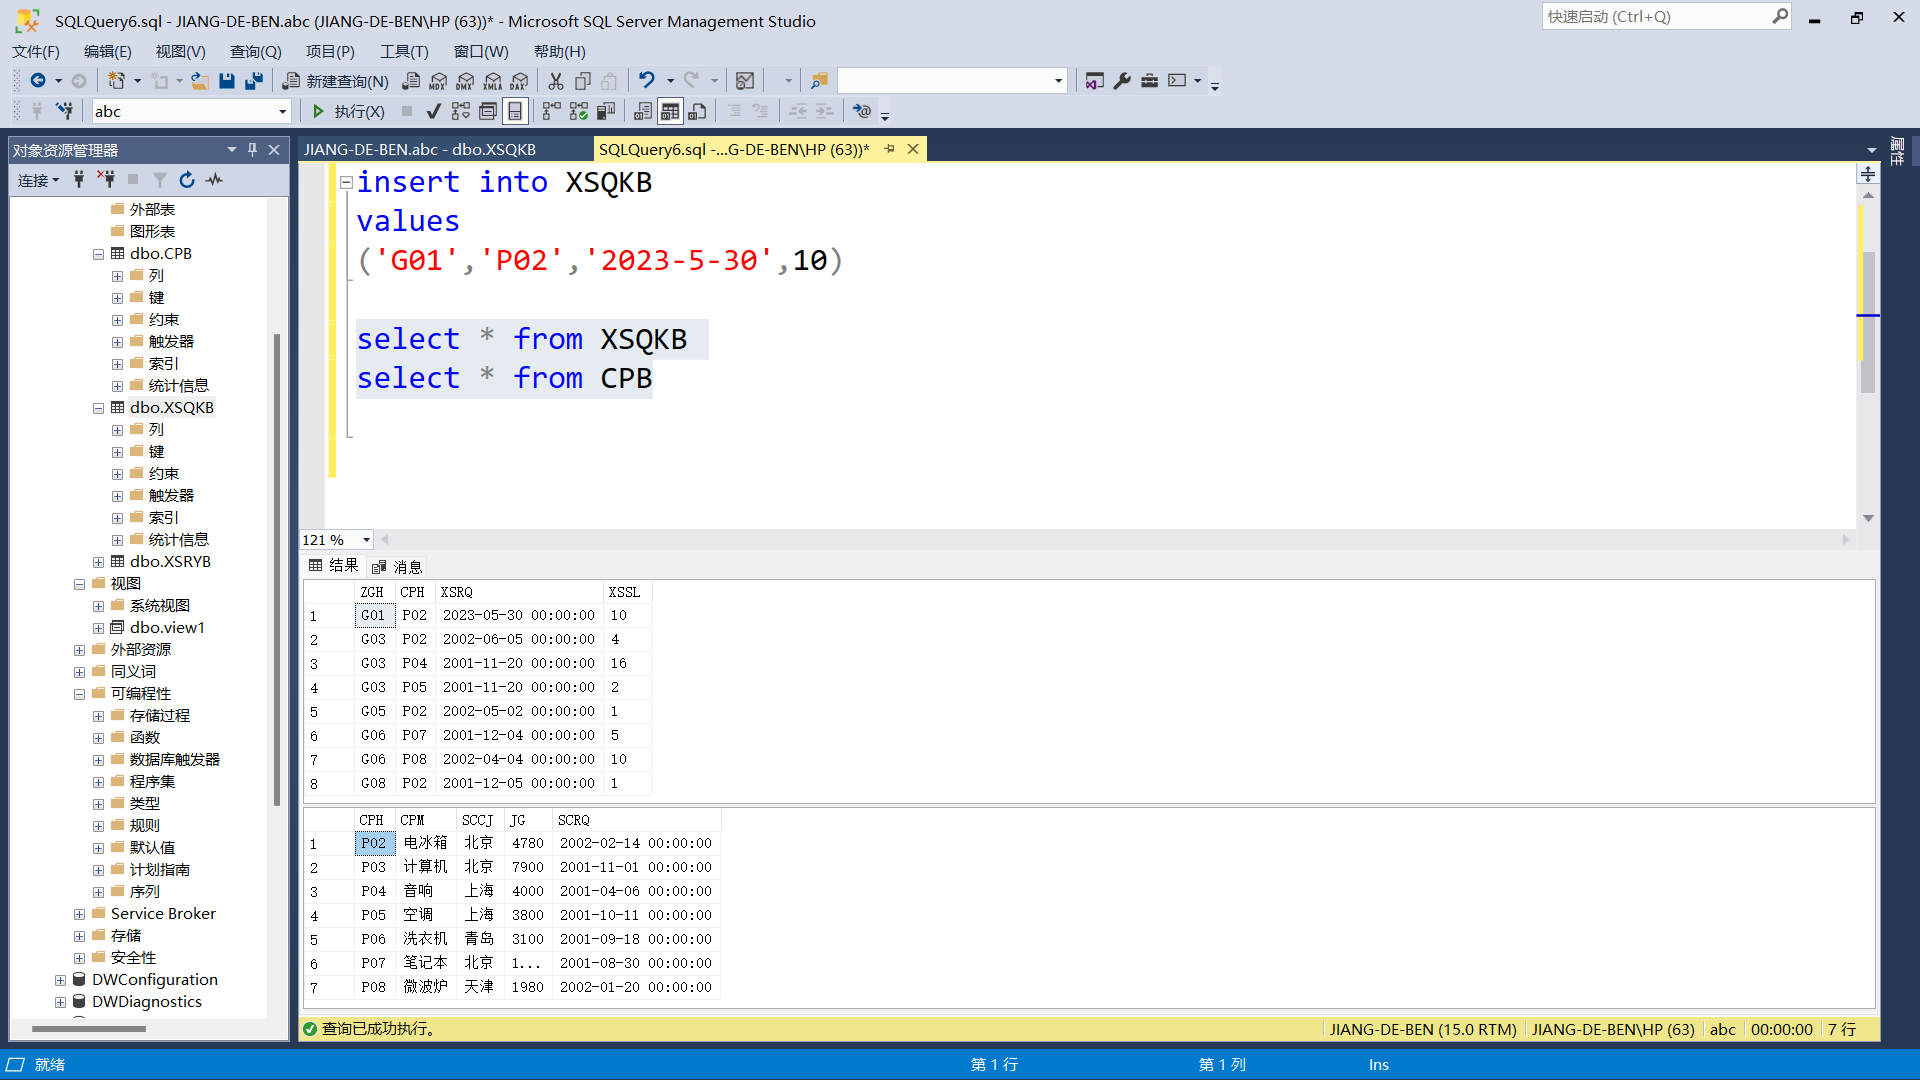
\includegraphics[width=0.9\linewidth]{img/6.png}
	\end{minipage}
    \caption{使用触发器查询结果}
\end{figure}

\newpage

\subsection{创建索引}
将100万行数据导入数据库,创建索引,比较引入索引前后的查询速度

将txt文件导入数据库如图所示
\begin{figure}[htbp]
	\centering
	\begin{minipage}{0.49\linewidth}
		\centering
		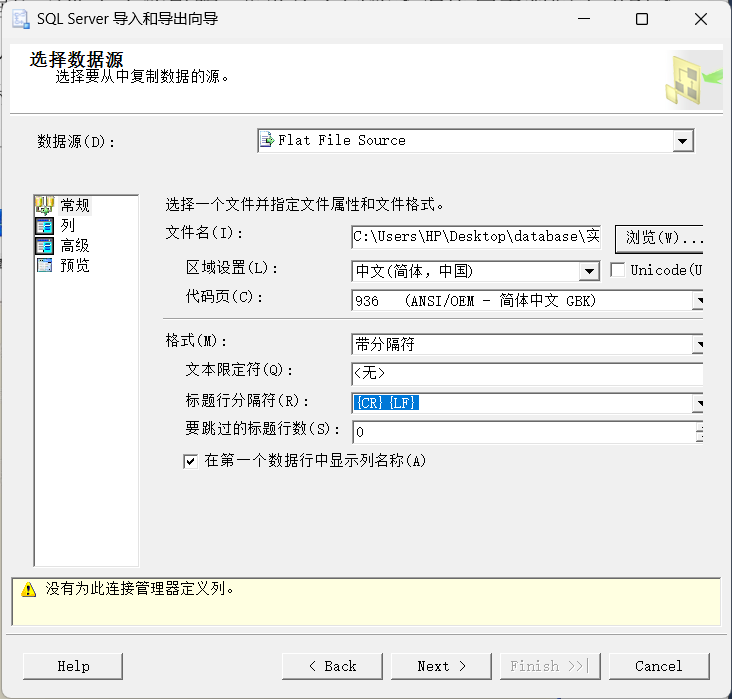
\includegraphics[width=0.9\linewidth]{img/7.png}
	\end{minipage}
	\begin{minipage}{0.49\linewidth}
		\centering
		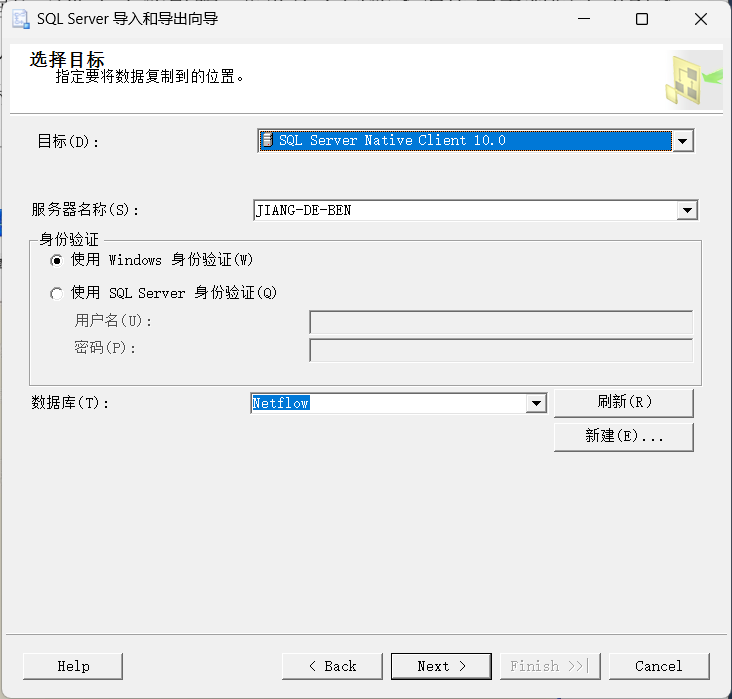
\includegraphics[width=0.9\linewidth]{img/8.png}
	\end{minipage}
    \caption{导入数据}
\end{figure}

使用select语句查询数据结果如下
\begin{figure}[htbp]
    \centering
    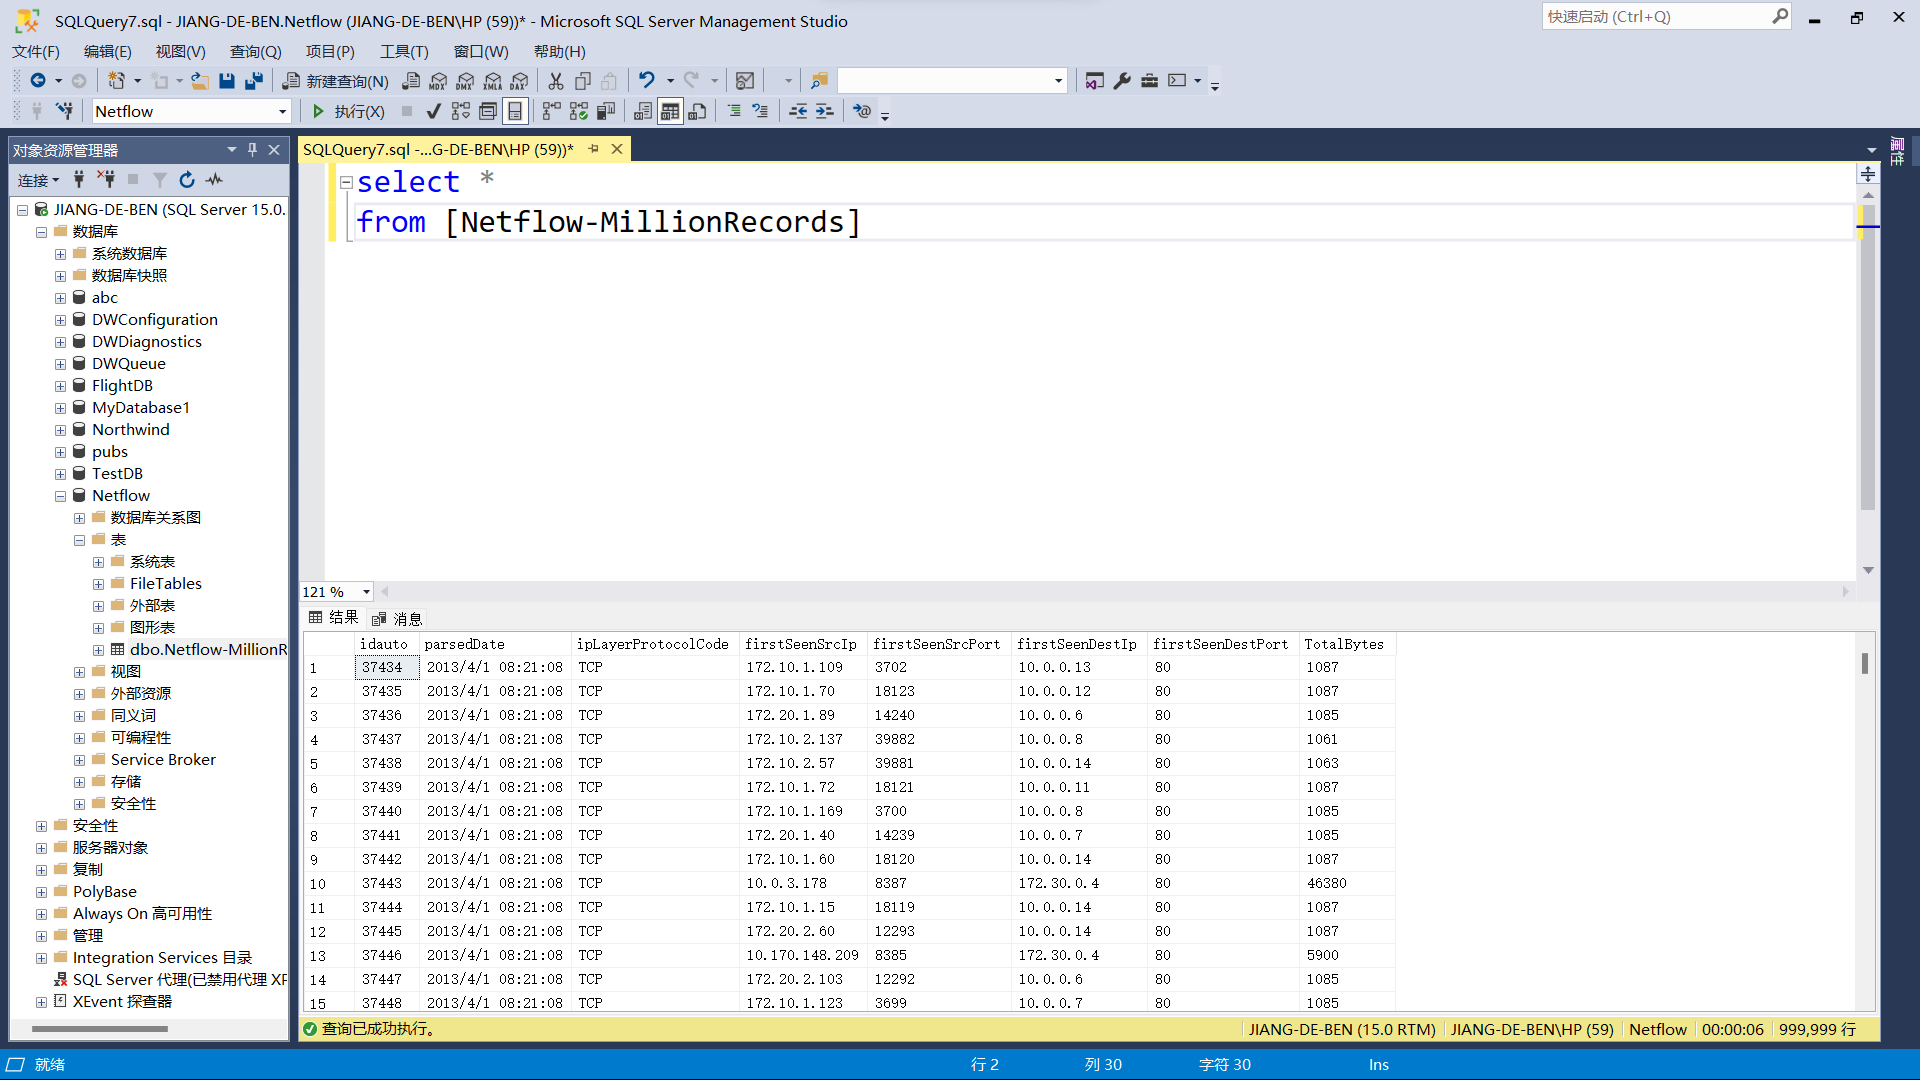
\includegraphics[width=0.8\textwidth]{img/10.png}
    \caption{查询数据}
\end{figure}



使用create index语句创建索引,代码如下:
\begin{lstlisting}[title=create index,frame=shadowbox]
    create clustered index netflow_s1
    on [Netflow-MillionRecords] (idauto)
    
    create index netflow_s2
    on [Netflow-MillionRecords] (ipLayerProtocolCode)
    
    create index netflow_s3
    on [Netflow-MillionRecords] (parsedDate)
\end{lstlisting}

创建索引前后数据库内存大小比较
\begin{figure}[htbp]
	\centering
	\begin{minipage}{0.49\linewidth}
		\centering
		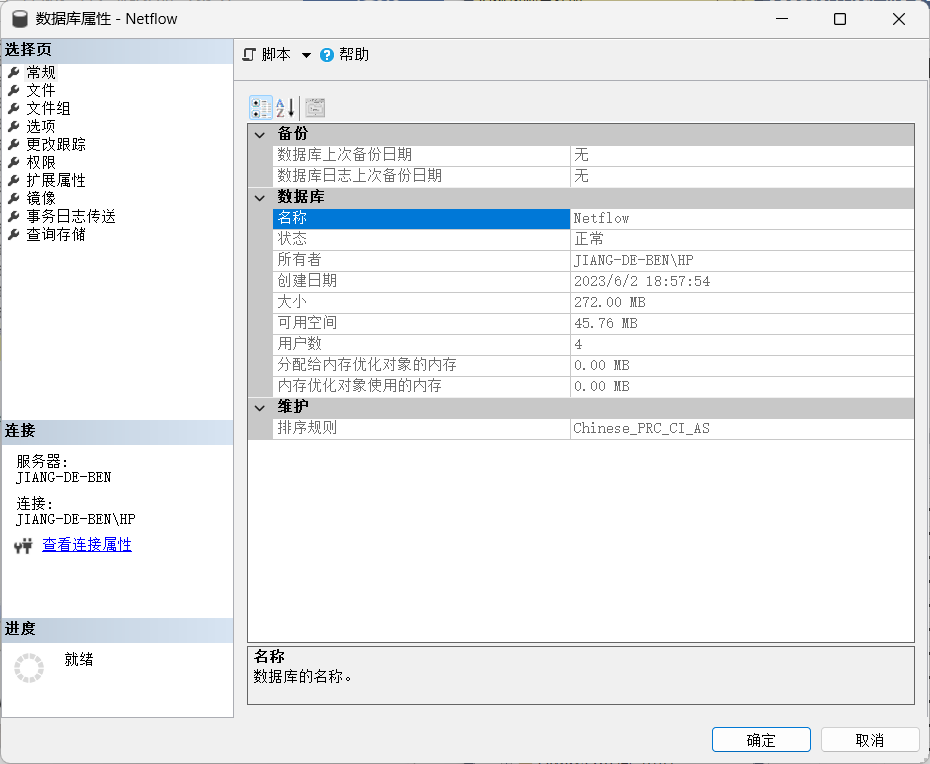
\includegraphics[width=0.9\linewidth]{img/11.png}
	\end{minipage}
	\begin{minipage}{0.49\linewidth}
		\centering
		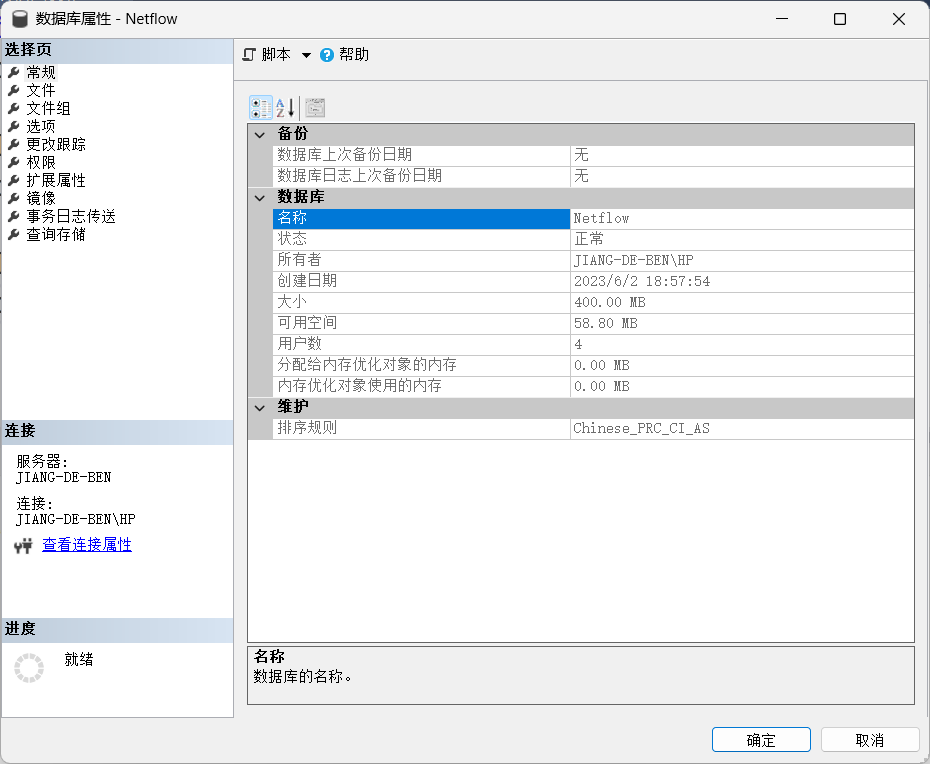
\includegraphics[width=0.9\linewidth]{img/12.png}
	\end{minipage}
    \caption{创建索引前后数据库内存大小比较}
\end{figure}

使用select语句查询数据结果如下
\begin{figure}[htbp]
    \centering
    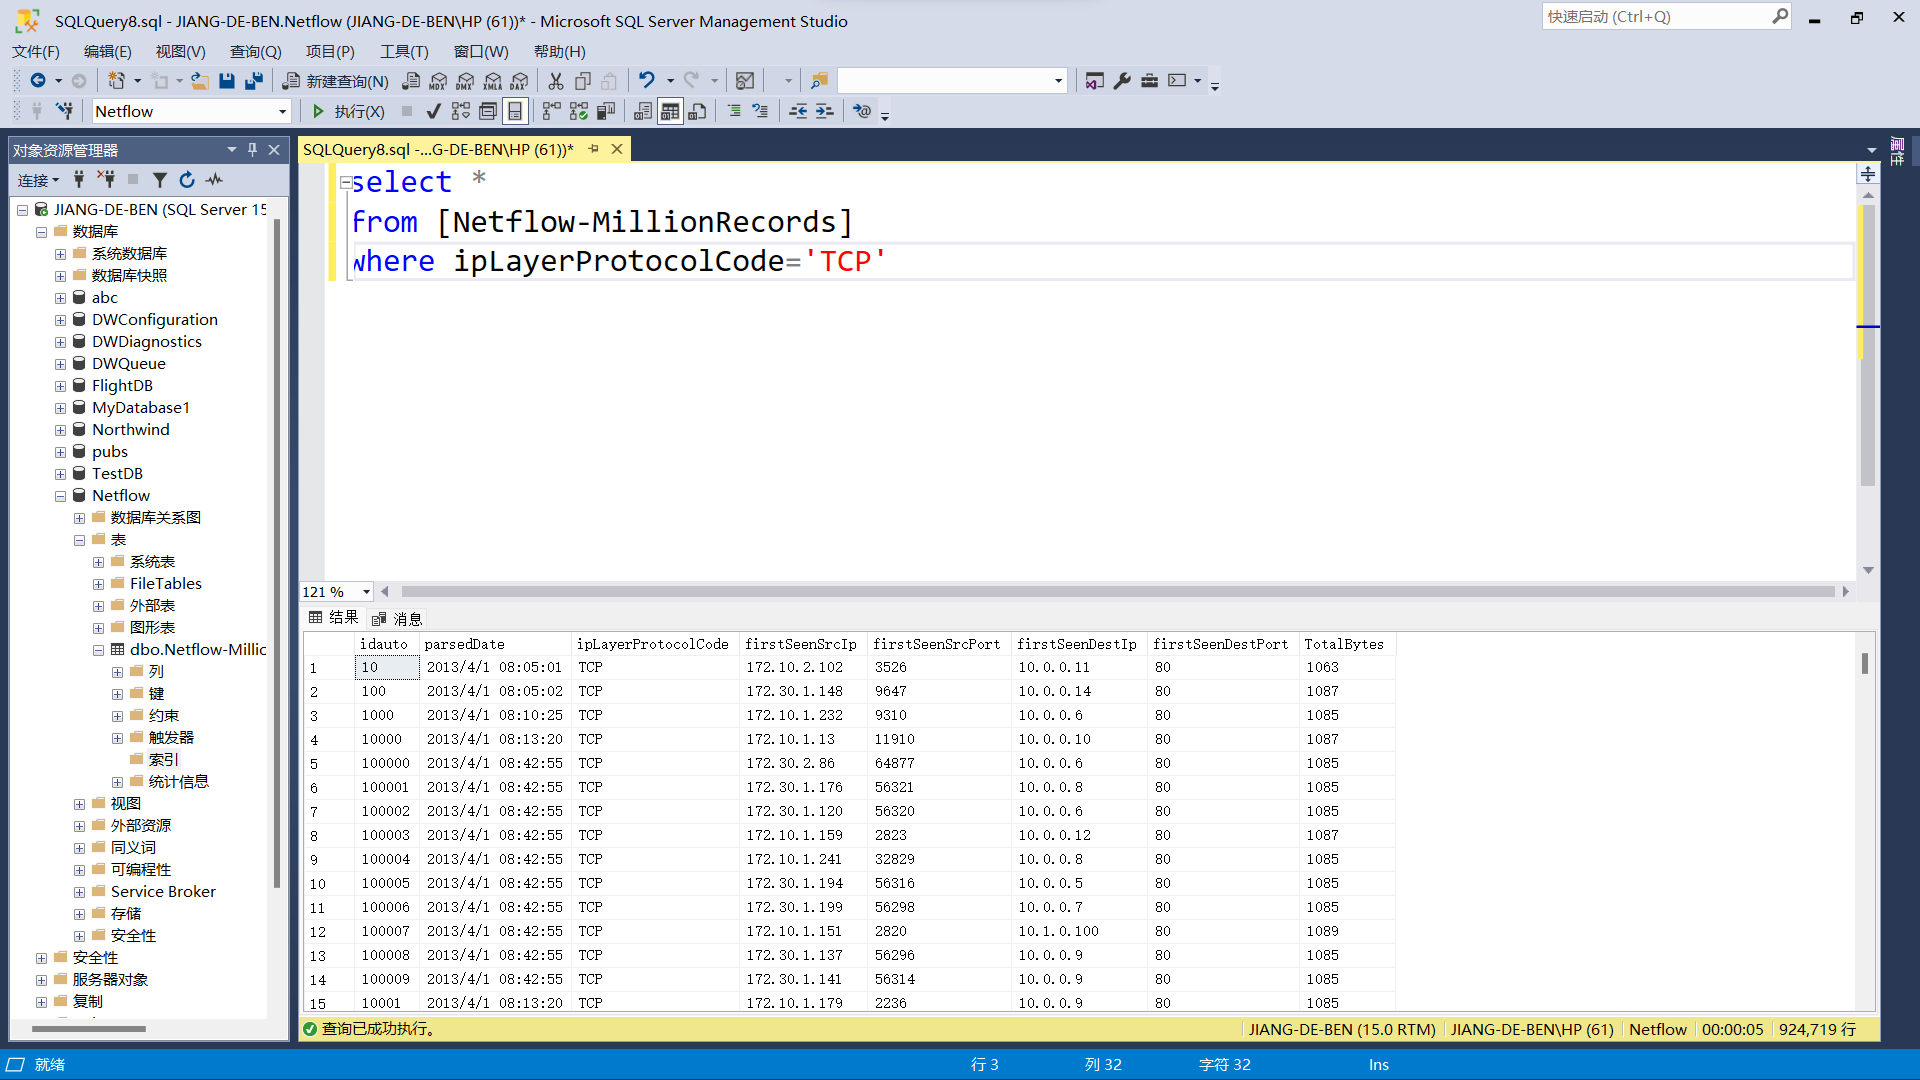
\includegraphics[width=0.8\textwidth]{img/13.png}
    \caption{查询数据}
\end{figure}

可以看出,创建索引后,数据库内存增加较多,在数据为100万行的时候,查询速度并没有很大差异,推测原因是数据量较小,查询速度并没有明显差异,同时SQL server的版本为2019,查询速度已经很快,所以创建索引对查询速度的影响不明显。但是当数据量增大时,查询速度会有明显差异。当数据量达到1000万行时,查询速度会有比较明显的差异。

\section{实验总结}
本次实验主要学习了视图、存储过程、游标、触发器、索引的使用方法,通过实验,我对这些知识有了更深的理解。

在创建视图的时候,视图的创建语句中,where子句中不能使用聚合函数,否则会报错;在创建存储过程的时候,存储过程中的变量必须先声明后使用,否则会报错;在创建游标的时候,游标的使用方法和C语言中的游标类似,都是先声明游标,然后打开游标,然后使用fetch next语句获取游标中的数据,最后关闭游标;在创建触发器的时候,触发器的创建语句中,for子句中可以使用insert、update、delete,表示在插入、更新、删除数据时触发器会被触发;在使用触发器的时候,触发器中的变量使用inserted表示插入的数据,使用deleted表示删除的数据,使用update表示更新的数据;

在创建索引的时候,使用了用空间换时间的思想,通过创建索引,可以提高查询速度,但是会增加数据库的内存占用。






\end{document}